\chapter{Desempe\~no del programa original}
\label{ch:prev_work}

A continuaci\'on se exponen los resultados de diferentes pruebas realizadas sobre el programa original con la finalidad de medir su desempe\~no computacional en t\'erminos de tiempo de ejecuci\'on y uso de memoria.
\bigskip

Estas pruebas se llevaron a cabo en un computador personal de 8 GB (DDR4) de RAM. La raz\'on de esta  medida (que no se hayan ejecutado en Leftraru) tuvo que ver con que el c\'odigo original contiene demasiadas l\'ineas con el comando \texttt{glob}\footnote{\url{https://docs.python.org/3.5/library/glob.html}} de Python el cual lista reiteradamente el contenido de los directorios de los archivos lo que finalmente termina saturando el nodo destinado para el lanzamiento del programa (ya que recorre la lista de 93 supernovas de HiTS, repitiendo para cada una de ellas el mismo proceso). Por esto \'ultimo, los administradores del sistema del NLHPC sugirieron modificaciones al programa original, sin embargo, en pos de continuar con el esp\'iritu de esta tesis, se opt\'o por efectuar los experimentos de manera local (usando un computador personal) evitando as\'i introducir m\'as modificaciones (se adapt\'o el programa para Python 3.5, ya que originalmente estaba para 2.7 agregando cambios menores como la forma de imprimir mensajes en consola (\texttt{print})).
\bigskip

La pipeline original (\texttt{candidate\_search}) est\'a estructurada, a grandes rasgos por dos bloques de \textbf{detecci\'on}: el primero est\'a destinado a buscar una supernova confirmada por HiTS (cuya coordenada es conocida) y el segundo a obtener la informaci\'on de otros posibles candidatos que se hayan encontrado anteriormente. Cabe recalcar que a este segundo proceso se ingresa s\'olo en el caso que se hayan encontrado candidatos desconocidos en primera fase.
\bigskip

El proceso de b\'usqueda de la supernova se inicializa en una instancia de \textsc{RunData}, \textbf{listando los archivos desde disco}, para preparar las im\'agenes y el resto de archivos que ser\'an usados para el proceso iterativo siguiente. 

\begin{enumerate}
\item \textbf{C\'alculo de flujo:} Es el primer paso del ciclo. A partir de las im\'agenes cient\'ificas y de calibraci\'on se obtiene el flujo (en ADU\footnote{Analog-to-digital unit}) por pixel y es registrado en una matriz (\texttt{numpy array}) en cada iteraci\'on. 
\item \textbf{Proceso de estimaci\'on con filtro de Kalman:} Corresponde a la segunda etapa del proceso de iteraci\'on. En ella se realizan los procesos de predicci\'on y correcci\'on para obtener una nueva estimaci\'on. 
\item \textbf{Detecci\'on de fuentes:} El tercer paso del ciclo. En \'el se estudia la idoneidad de los pixeles tanto del flujo como de las estimaciones del mismo (obtenidos con el filtro de Kalman) y del resto de las im\'agenes al momento de verificar una serie de criterios con los cuales estos mismos se agrupar\'ian  entre vecinos para formar potenciales candidatos.  
\item \textbf{Actualizaci\'on de candidatos:} Revisa si hay nuevos candidatos a ser considerados. Se registran en un arreglo (\texttt{numpy array}).
\end{enumerate}

Si en el proceso anterior se encontr\'o alg\'un candidato, se procede a repetir los pasos de obtenci\'on de flujos, estimaciones y filtrado de pixeles. La diferencia est\'a en que en esta oportunidad de van guardando los resultados en una estructura de datos de diccionario. El nuevo ciclo queda como sigue:

\begin{enumerate}
\item \textbf{C\'alculo de flujo:} Repite el primer paso del ciclo descrito anteriormente.
\item \textbf{Proceso de estimaci\'on con filtro de Kalman:} Repite el segundo paso del ciclo descrito anteriormente.
\item \textbf{Detecci\'on de fuentes:} Realiza el mismo proceso que el tercer paso del ciclo anterior.
\item \textbf{Guardado de resultados:} La informaci\'on de los nuevos candidatos encontrados previamente es guardado en una estructura de diccionario y registrado en discomo con un formato NPZ (\textsc{NumPy}).
\end{enumerate}


El diagrama de la figura \ref{fig:des_sif} entrega una perspectiva general de la secuencia de pasos que realiza el programa.
\bigskip

Cabe destacar que durante el proceso de refactoring del programa original se encontr\'o que la lista de archivos, que debe ser procesada en orden de acuerdo a la \'epoca (o fecha de observaci\'on) no estaban siendo bien ordenadas durante el proceso de selecci\'on de im\'agenes cient\'ificas a partir del valor de \texttt{airmass} en la clase \textsc{FitsHandler}.
\bigskip


\begin{figure}[h!]
\centering
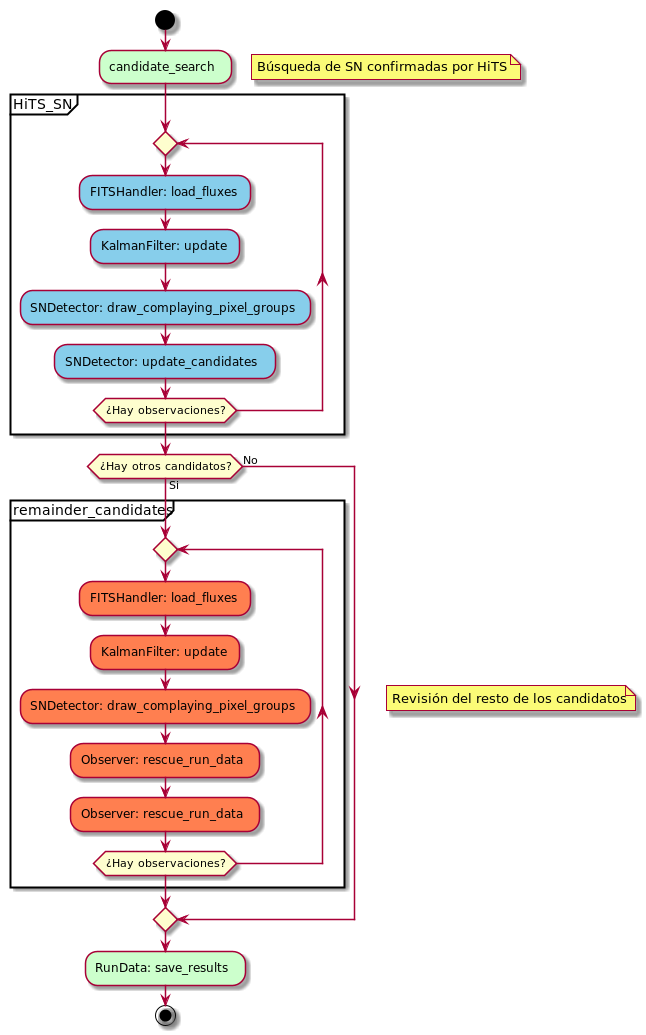
\includegraphics[scale=.5]{images/results/sif_act}
\caption{Diagrama de actividad del programa original. Se aprec\'ian dos ciclos principales: el primero est\'a destinado a la b\'usqueda de una supernova de HiTS, y el segundo a la revisi\'on de la lista de posibles candidatos encontrados durante la verificaci\'on de la supernova de HiTS. Notar que hay pasos que se repiten en la realizaci\'on de ambos an\'alisis.}
\label{fig:des_sif}
\end{figure}

\section{Tiempo de ejecuci\'on}

El estudio del tiempo de ejecuci\'on del programa se realiz\'o usando la funci\'on \texttt{getrusage} de la librer\'ia \texttt{resource} de Python, midiendo el tiempo de usuario en segundos. Las mediciones se realizaron sobre tres conjuntos de datos (las cuales contienen alguna supernova detectada por HiTS) seleccionados al azar: SN14, SN18 y  SN80. En cada uno de ellos comprende secuencias de 26, 23 y 18 observaciones respectivamente. 

\begin{table}[h!]
\centering
\begin{tabular}{|l|l|l|l|l|}
\hline
\textbf{ID} & \textbf{C\'alc. Flujos [s]} & \textbf{Aplic. KF [s]} &  \textbf{Agrup. Pixeles [s]}  & \textbf{Actual. Candidatos [s]}\\ \hline \hline
SN14        & 293.91            & 24.90        &  68.30 & 0.02 \\ \hline
SN18            & 260.09             & 22.56         &  45.52  & 0.00\\ \hline
SN80            & 204.93             & 17.69         &   38.21 & 0.00 \\ \hline \hline
%Media & 303.08 &  26.23 & 37.83 & 0.01\\\hline 
$\bar{t}/Obs$ & 11.00 &  0.97 & 2.24 & 0.00\\\hline 
\end{tabular}
\label{tab:t1}
\caption{Resultados de tiempos de ejecuci\'on correspondientes a calculo de flujos, estimaci\'on de los filtros, agrupaci\'on de pixeles y filtrado de los mismos durante el peri\'odo de reconocimiento de la supernova correspondiente. Para esta prueba se utiliz\'o el filtro de Kalman B\'asico. La \'ultima fila corresponde a la media por observaci\'on.}
\end{table}

\begin{table}[h!]
\centering
\begin{tabular}{|l|l|l|l|l|}
\hline
\textbf{ID} & \textbf{C\'alc. Flujos [s]} & \textbf{Aplic. KF [s]} &  \textbf{Agrup. Pixeles [s]}  & \textbf{Guardar resultados [s]}\\ \hline \hline
SN14        & 303.18            & 27.28        &  72.34 & 0.02 \\ \hline
SN18            & 0.00             & 0.00         &  0.00  & 0.00\\ \hline
SN80            & 0.00             & 0.00         &   0.00 & 0.00 \\ \hline\hline 
%Media & 306.98 &  28.89 & 38.89  & 0.07\\\hline 
$\bar{t}/Obs$ & 11.66 &  1.05 & 2.78 & 0.00\\\hline 
\end{tabular}
\label{tab:t2}
\caption{Resultados de tiempos de ejecuci\'on correspondientes a calculo de flujos, estimaci\'on de los filtros, agrupaci\'on de pixeles y filtrado de los mismos durante el peri\'odo de estudio de los nuevos candidatos encontrados en el paso anterior. Para esta prueba se utiliz\'o el filtro de Kalman B\'asico. Se observa que para las dos \'ultimas supernovas los tiempos son cero ya que no se encontraron m\'as candidatos.}
\end{table}


\begin{table}[h!]
\centering
\begin{tabular}{|l|l|l|l|l|}
\hline
\textbf{ID} & \textbf{C\'alc. Flujos [s]} & \textbf{Aplic. KF [s]} &  \textbf{Agrup. Pixeles [s]}  & \textbf{Actual. Candidatos [s]}\\ \hline \hline
SN14        & 342.44            & 798.48        &  76.47 & 0.00 \\ \hline
SN18            & 273.64             & 566.89         &  47.96  & 0.00\\ \hline
SN80            & 210.68             & 420.12         &   36.05 & 0.00 \\ \hline \hline 
%Media & 309.32 & 638.48 &  37.07 & 0.01\\\hline
$\bar{t}/Obs. $& 12.25 & 26.23 & 2.34 & 0.00\\\hline 
\end{tabular}
\label{tab:t3}
\caption{Resultados de tiempos de ejecuci\'on correspondientes a calculo de flujos, estimaci\'on de los filtros, agrupaci\'on de pixeles y filtrado de los mismos durante el peri\'odo de reconocimiento de la supernova correspondiente. Para esta prueba se utiliz\'o el filtro de Kalman de M\'axima Correntrop\'ia.}
\end{table}

\begin{table}[h!]
\centering
\begin{tabular}{|l|l|l|l|l|}
\hline
\textbf{ID} & \textbf{C\'alc. Flujos [s]} & \textbf{Aplic. KF [s]} &  \textbf{Agrup. Pixeles [s]}  & \textbf{Guardar resultados [s]}\\ \hline \hline
SN14        & 307.64            & 680.65        &  65.67 & 0.02 \\ \hline
SN18            & 0.00             & 0.00         &  0.00  & 0.00\\ \hline
SN80            & 0.00             & 0.00         &   0.00 & 0.00 \\ \hline \hline
%Media & 306.71 & 634.09 &  36.34 & 0.05\\\hline
$\bar{t}/Obs. $& 11.83 & 26.18 & 2.53 & 0.00\\\hline  
\end{tabular}
\label{tab:t4}
\caption{Resultados de tiempos de ejecuci\'on correspondientes a calculo de flujos, estimaci\'on de los filtros, agrupaci\'on de pixeles y filtrado de los mismos durante el peri\'odo de estudio de los nuevos candidatos encontrados en el paso anterior. Para esta prueba se utiliz\'o el filtro de Kalman de M\'axima Correntrop\'ia. Se observa que para las dos \'ultimas supernovas los tiempos son cero ya que no se encontraron m\'as candidatos.}
\end{table}

\begin{table}[h!]
\centering
\begin{tabular}{|l|l|l|l|}
\hline
\textbf{ID} & \textbf{B\'usqueda SN [s]} & \textbf{Revisi\'on candidatos[s]} & \textbf{Tiempo total [s]} \\ \hline
\hline
SN14 & 387.13 & 402.82 & 789.95 \\\hline
SN18 & 328.17 & 0.00 & 328.17\\\hline
SN80 & 260.83 & 0.00 & 260.83 \\\hline\hline
%Media & 367.15 & 374.83 & 741.98  \\\hline
 $\bar{t}/Obs. $& 14.55 & -- & --\\\hline 
\end{tabular}
\label{tab:t5}
\caption{Tiempo de ejecuci\'on de los procesos de b\'usqueda de supernova de HiTS, revisi\'on de los candidatos encontrados y tiempo total comprendido por ambos procesos usando filtro de Kalman B\'asico. La \'ultima fila corresponde a tiempo total promedio por observaci\'on.}
\end{table}


\begin{table}[h!]
\centering
\begin{tabular}{|l|l|l|l|}
\hline
\textbf{ID} & \textbf{B\'usqueda SN [s]} & \textbf{Revisi\'on candidatos [s]} & \textbf{Tiempo total [s]} \\ \hline
\hline
SN14 & 1217.39 & 1053.98 & 2068.80\\\hline
SN18 & 888.49 & 0.00 & 0.00\\\hline
SN80 & 666.85 & 0.00& 0.00\\\hline \hline
 $\bar{t}/Obs. $& 40.83 & -- & --\\\hline 
\end{tabular}
\label{tab:t6}
\caption{Tiempo de ejecuci\'on de los procesos de b\'usqueda de supernova de HiTS, revisi\'on de los candidatos encontrados y tiempo total comprendido por ambos procesos usando filtro de Kalman de M\'axima correntrop\'ia.}
\end{table}

\section{Uso de memoria}

La memoria ocupada por el programa se midi\'o en t\'erminos de MiB (Mebibyte) usando la librer\'ia \texttt{memory\_profiler}. Posteriormente las mediciones en la unidad previamente mencionada fueron pasadas a MB\footnote{$1MiB\simeq 1.049MB$ }

\begin{figure}[h!]
\centering
\subfloat[Memoria ocupada en SN14]{\label{fig:kbf_14}{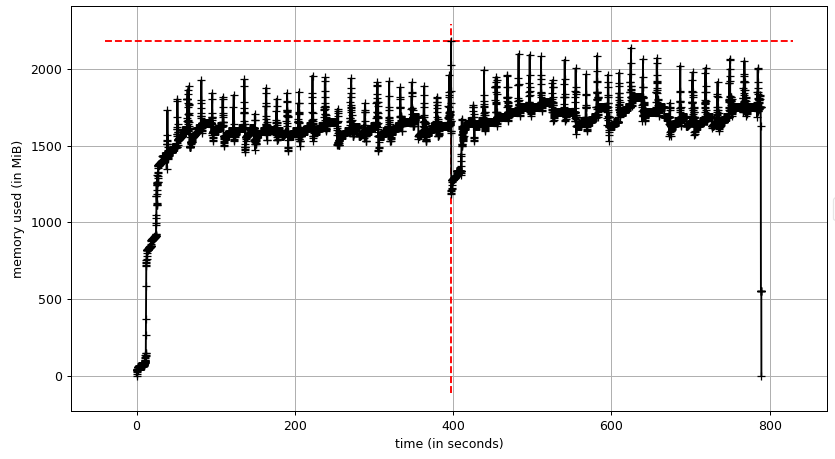
\includegraphics[width=0.5\textwidth]{images/results/sn14_00}}}\hfill
\subfloat[Memoria ocupada en SN18]{\label{fig:kbf_18}{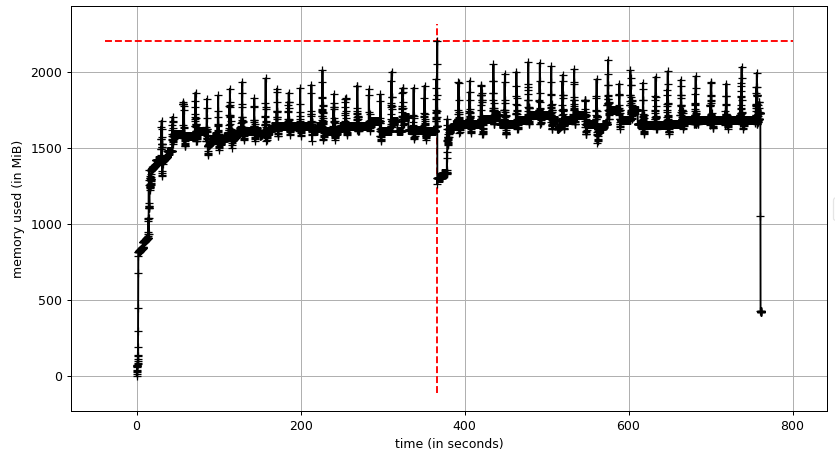
\includegraphics[width=0.5\textwidth]{images/results/sn18_00}}}\vfill
\subfloat[Memoria ocupada en SN80]{\label{fig:kbf_80}{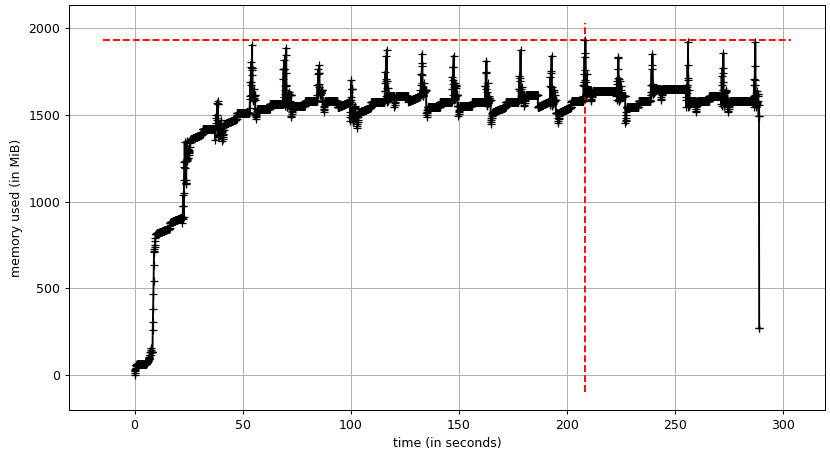
\includegraphics[width=0.5\textwidth]{images/results/sn80_00}}}
\caption{Comportamiento de la memoria (en mebibytes) durante la ejecuci\'on para los tres conjuntos de datos. En los tres lanzamientos se us\'o el filtro de Kalman B\'asico.}
\label{fig:mem_kbf}
\end{figure}

\begin{table}[h!]
\centering
\begin{tabular}{|l|l|}
\hline
\textbf{ID} & Memoria [MB]\\\hline\hline
SN14 & 2282.42\\\hline
SN18 & 2063.02\\\hline
SN80 & 2021.27\\\hline
\end{tabular}
\caption{Memoria principal (en unidades de MB) usada durante la ejecuci\'on del programa original usando la versi\'on b\'asica del filtro de Kalman.}
\label{tab:mem1}
\end{table}

\begin{figure}[h!]
\centering
\subfloat[Memoria ocupada en SN14]{\label{fig:mc_14}{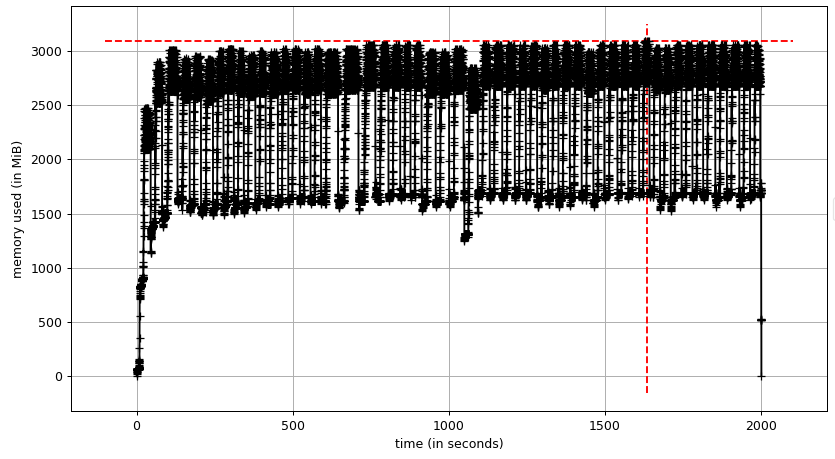
\includegraphics[width=0.5\textwidth]{images/results/sn14_01}}}\hfill
\subfloat[Memoria ocupada en SN18]{\label{fig:mc_18}{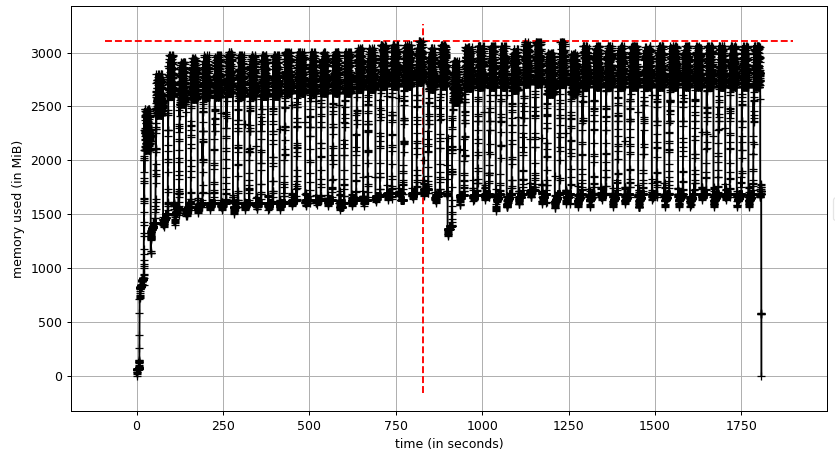
\includegraphics[width=0.5\textwidth]{images/results/sn18_01}}}\vfill
\subfloat[Memoria ocupada en SN80]{\label{fig:mc_80}{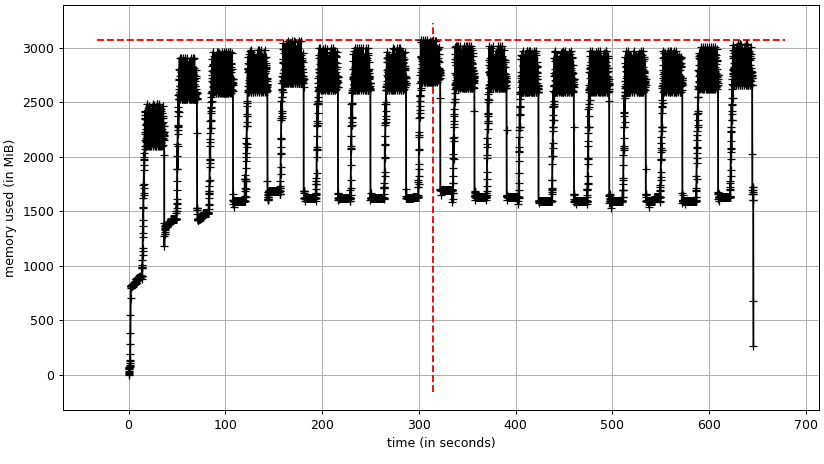
\includegraphics[width=0.5\textwidth]{images/results/sn80_01}}}
\caption{Comportamiento de la memoria (en mebibytes) durante la ejecuci\'on para los tres conjuntos de datos. En los tres lanzamientos se us\'o el filtro de Kalman de correntrop\'ia m\'axima.}
\label{fig:mem_mcc}
\end{figure}

\begin{table}[h!]
\centering
\begin{tabular}{|l|l|}
\hline
\textbf{ID} & Memoria [MB]\\\hline\hline
SN14 & 3353.13\\\hline
SN18 & 3194.96\\\hline
SN80 & 3209.67\\\hline
\end{tabular}
\caption{Memoria principal (en unidades de MB) usada durante la ejecuci\'on del programa original usando filtro de Kalman de m\'axima correntrop\'ia.}
\label{tab:mem2}
\end{table}

\section{Falsos negativos y verdaderos positivos}
La siguiente tabla (\ref{tab:tpfn}), muestra el resultado de la detecci\'on de las 93 supernovas de HiTS para el conjunto de datos del a\~no 2015. Esta prueba fue realizada en Leftraru en junio del presente a\~no (previo a cambios introducidos por autor original). 
\begin{table}[h!]
\centering
\begin{tabular}{|l|l|l|}
\hline
\textbf{Filtro} & \textbf{TP} & \textbf{FN} \\ \hline
Básico          & 41          & 52          \\ \hline
MCC             & 41          & 52          \\ \hline
\end{tabular}
\caption{N\'umero de falsos negativos y verdaderos positivos encontrados usando cada uno de los filtros. No se observan diferencias sustanciales entre los resultados de cada filtro.}
\label{tab:tpfn}
\end{table}

Estableciendo par\'ametros de umbral de 200.0 para flujo y de 50.0 para la velocidad de flujo (cantidades estimadas por el filtro de Kalman) se obtienen resultados id\'enticos para ambos filtros al momento de detectar supernovas conocidas por HiTS. En ambos casos se detectaron 41 de 93, lo que da un porcentaje de 44\%.
\bigskip

Sin embargo, cabe destacar que dentro de las 93 supernovas, existen 36 de las cuales se conoce que corresponden a supernovas j\'ovenes que se encuentran en pleno periodo de aumento de luminosidad (todas del a\~no 2015). De estas 36, para ambos filtros, se detectaron 26 lo que corresponder\'ia a un 72\%. Por esta raz\'on se pretende que el desarrollo de un nuevo filtro de aproximaci\'on no-lineal podr\'ia entregar esperanzas de mejorar este resultado.
\bigskip

\section{Falsos positivos}
El poder reconocer falsos positivos a trav\'es de este algoritmo se hace imposible si no se cuenta con una herramienta externa de visualizaci\'on o de machine learning (por ejemplo, usando un clasificador de conjuntos de pixeles que eval\'ue la probabilidad de que se trata efectivamente de una supernova joven). Esto se debe a que existen variados objetos como estrellas variables o \textit{artefactos} que corresponden a zonas ruidosas de la imagen  cient\'ifica (en particular, bordes) y pueden proveer valores alterados de flujo lo que en algunos casos puede conllevar a la detecci\'on de falsos positivos.
\bigskip

Una forma de poder estudiar un falso positivo es a trav\'es de la visualizaci\'on de su espacio de fase y la obtenci\'on de su curva entr\'opica.